\documentclass[prd, superscriptaddress, tightenlines, longbibliography, nofootinbib, eqsecnum, amsfonts, amsmath, floatfix, twocolumn, notitlepage]{revtex4-2}
\pdfoutput=1
\usepackage{ftnxtra}
%\usepackage{footmisc}
\usepackage[utf8]{inputenc}
\usepackage{mathrsfs}
\usepackage{euscript}
\usepackage{graphics}
\usepackage{graphicx}
\usepackage{amsmath}
\usepackage{amssymb}
\usepackage{gensymb}
\usepackage{tabularx}
\usepackage{subfigure}
%\usepackage{subcaption}
\usepackage{bm}
\usepackage[usenames,dvipsnames,svgnames,table]{xcolor}
\definecolor{linkcolor}{rgb}{0.6,0,0}
\definecolor{citecolor}{rgb}{0,0,0.75}
\definecolor{urlcolor}{rgb}{0.12,0.46,0.7}
\usepackage{xspace}
\usepackage{wasysym}
\usepackage{times}
\usepackage{appendix}
\usepackage{comment}
\usepackage{lipsum}
\usepackage[nolist,nohyperlinks]{acronym}
\usepackage{float}
\usepackage{simplewick}
\usepackage{natbib, ifthen}
\usepackage[breaklinks, colorlinks, urlcolor=urlcolor, linkcolor=linkcolor,citecolor=citecolor,pdfencoding=auto]{hyperref}
%\usepackage{longtable}
%\usepackage{booktabs} % for tables
\usepackage{listings}
\interfootnotelinepenalty=1000000
\newcommand{\apjs} {Astrophys. J. Suppl.}
\usepackage{caption}

\newcommand{\orcid}[1]{{\sc ORCiD:} \href{https://orcid.org/#1}{#1}}
\newcommand{\orcidacronym}[2]{\href{https://orcid.org/#2}{#1}}
\newcommand{\ALorcid}{\orcidacronym{AL}{0000-0001-5927-6667}}

\newcommand{\la}{\langle}
\newcommand{\ra}{\rangle}

\newcommand{\onesig}[1]{(68\%, \text{#1})}
\newcommand{\twosig}[1]{(95\%, \text{#1})}
\newcommand{\twoonesig}[3]{
\begin{equation}
\left.
 \begin{aligned}
#1 \\ #2
 \end{aligned}
\ \right\} \ \ \mbox{\text{#3}}
\end{equation}
}
\newcommand{\twotwosig}[3]{
\begin{equation}
\left.
 \begin{aligned}
#1 \\ #2
 \end{aligned}
\ \right\} \ \ \mbox{95\%, \text{#3}}
\end{equation}
}


\newcommand{\fsky}{f_{\rm sky}}


\providecommand{\planck}{\textit{Planck}}
\providecommand{\Planck}{\planck}
\newcommand{\camspec}{{\tt CamSpec}}
\newcommand{\plik}{{\tt Plik}}
\newcommand{\commander}{{\tt Commander}}
\newcommand{\mspec}{{\tt MSPEC}}
\newcommand{\smica}{{\tt SMICA}}

\newcommand{\MCNzero}{\textrm{MC-}N^{(0)}}
\newcommand{\RDNzero}{\textrm{RD-}N^{(0)}}
\newcommand{\RDNone}[0]{\textrm{RD-}N^{(1)}}
\newcommand{\xpRDNone}[0]{\textrm{xpRD-}N^{(1)}}
\newcommand{\MCNone}[0]{\textrm{MC-}N^{(1)}}

\newcommand{\CFHTLENS}{CFHTLenS}
\newcommand{\meanchisquare}{\overline{\chi^2}}

\newcommand{\mksym}[1]{\ifmmode {\rm #1}\else #1\fi}
\newcommand{\dataplus}{{+}}
\newcommand{\WP}{\mksym{WP}}
\newcommand{\highL}{\mksym{highL}}
\newcommand{\BAO}{\mksym{BAO}}
\newcommand{\lensing}{\mksym{lensing}}
\newcommand{\ext}{\mksym{ext}}
\newcommand{\planckonly}{\planck}
\newcommand{\TT}{\mksym{TT}}
\newcommand{\TTTEEE}{\mksym{TT,TE,EE}}
\newcommand{\planckTTonly}{\planck\ \TT}
\newcommand{\planckTTTEEEonly}{\planck\ \TTTEEE}
\newcommand{\lowTEB}{\mksym{lowP}}
\newcommand{\lowEB}{\mksym{lowP}}
\newcommand{\WMAPTEB}{\lowTEB\dataplus\mksym{WP}}
\newcommand{\lowTP}{\mksym{lowT,P}}
\newcommand{\planckTT}{\planckTTonly\dataplus\lowTEB}
\newcommand{\planckall}{\planckTTTEEEonly\dataplus\lowTEB}
\newcommand{\planckTTBAO}{\planckTT\dataplus\BAO}
\newcommand{\planckTTlensing}{\planckTT\dataplus\lensing}
\newcommand{\planckallBAO}{\planckall\dataplus\BAO}
\newcommand{\planckalllensing}{\planckall\dataplus\lensing}
\newcommand{\planckTTlensext}{\planckTT\dataplus\lensing\dataplus\ext}
\newcommand{\datalabel}[1]{#1}

\newcommand{\shortTT}{\TT\dataplus\lowTEB}
\newcommand{\shortall}{\TTTEEE\dataplus\lowTEB}

\newcommand{\HighL}{\highL}

\newcommand{\As}{A_{\rm s}}
\newcommand{\At}{A_{\rm t}}
\newcommand{\nt}{n_{\rm t}}
\newcommand{\ns}{n_{\rm s}}
\newcommand{\lcdm}{{$\rm{\Lambda CDM}$}}
\newcommand{\rpivot}{r_{0.05}}
\newcommand{\rzerotwo}{r_{0.002}}
\newcommand{\Alens}{A_{\rm L}}
\newcommand{\Aphiphi}{A_{\rm L}^{\phi\phi}}
\newcommand{\omegak}{\Omega_K}
\newcommand{\omegal}{\Omega_\Lambda}
\newcommand{\alphaiso}{\alpha}

%\newcommand{\nrun}{n_{\text{run}}}
\newcommand{\thetaMC}{\theta_{\rm MC}}
\newcommand{\nrun}{d \ns / d\ln k}
\newcommand{\nrunfrac}{\frac{d \ns}{d\ln k}}
\newcommand{\zre}{z_{\text{re}}}
\newcommand{\yhe}{Y_{\text{P}}}
\newcommand{\ypbbn}{Y_{\text{P}}^{\rm BBN}}
\newcommand{\zeq}{z_{\text{eq}}}
\newcommand{\nnu}{N_{\rm eff}}
\newcommand{\neff}{\nnu}
\newcommand{\mnu}{\sum m_\nu}
\newcommand{\sumnu}{\sum m_\nu}
\newcommand{\mnusterile}{m_{\nu,\, \mathrm{sterile}}^{\mathrm{eff}}}
\newcommand{\meffsterile}{\mnusterile}
\newcommand{\Tactive}{T_{\mathrm{a}}}
\newcommand{\Tsterile}{T_{\mathrm{s}}}
\newcommand{\msthermal}{m_{\rm sterile}^{\rm thermal}}
\newcommand{\msDW}{m_{\rm sterile}^{\rm DW}}

\newcommand{\zdrag}{z_{\rm drag}}
\newcommand{\rdrag}{r_{\rm drag}}
\newcommand{\zstar}{z_{\ast}}
\newcommand{\rstar}{r_{\ast}}
\newcommand{\rs}{r_{\rm s}}
\newcommand{\thetastar}{\theta_{\ast}}
\newcommand{\DAstar}{D_{\rm A}}
\newcommand{\keq}{k_{\rm eq}}
\newcommand{\Ailensbestfit}{A_i^{\mbox{\scriptsize{theory}}}}
\newcommand{\Alensbestfit}{A^{\mbox{\scriptsize{theory}}}}
\newcommand{\DVBAO}{D_{\rm V}}
\newcommand{\DA}{D_{\rm A}}


%\newcommand{\zeq}{z_{\rm eq}}


\newcommand{\fixme}[1]{{\color{Red}{ FIXME: #1}}}
\newcommand{\quietfixme}[1]{{\color{Red} #1}}
\newcommand{\notate}[1]{{\color{olive} NOTE: #1}}

\newcommand{\fnl}{\ensuremath{f_{\text{NL}}}}

\newcommand{\taunl}{\ensuremath{{\tau_{\text{NL}}}}}

\newcommand{\gnl}{\ensuremath{g_{\text{NL}}}}

% tauNL-estimator
\newcommand{\htaunl}{\ensuremath{{\hat{\tau}_{\rm NL}}}}


\newcommand{\fnlloc}{f^{\rm local}_{\rm NL}}
\newcommand{\fnleqi}{f^{\rm equil}_{\rm NL}}

\providecommand{\Planck}{\textit{Planck}}
\providecommand{\planck}{\Planck}
\newcommand{\covinvT}{\bar{\Theta}}
\newcommand{\Ltemp}{\tilde{T}}
\newcommand{\lensedC}{\tilde{C}}
\newcommand{\Lmin}{{L_{\rm min}}}

%\providecommand{\lea}{\lesssim}
%\providecommand{\gea}{\gtrsim}
\providecommand{\lea}{\la}
\providecommand{\gea}{\ga}


\providecommand{\alt}{\lea}
\providecommand{\agt}{\gea}
\providecommand{\text}[1]{\rm{#1}}



\newcommand{\Msun}{M_\odot}
\newcommand{\tot}{{\text{tot}}}
\newcommand{\Mpc}{\text{Mpc}}
\newcommand{\half}{{\textstyle \frac{1}{2}}}
\newcommand{\third}{{\textstyle \frac{1}{3}}}
\newcommand{\numfrac}[2]{{\textstyle \frac{#1}{#2}}}
\renewcommand{\d}{\text{d}}
\newcommand{\grad}{\nabla}
\newcommand{\km}{{\rm{\,km\,}}}

\newcommand{\Hunit}{\text{km}\,\text{s}^{-1}\,\Mpc^{-1}}
\newcommand{\Gyr}{{\rm Gyr}}
\providecommand{\muK}{\mu{\rm K}}
\providecommand{\arcmin}{{\rm arcmin}}
\newcommand{\muKarcmin}{\,\muK\,\arcmin}
\newcommand{\muKsq}{(\mu\rm{K})^2}
\newcommand{\lmax}{l_{\text{max}}}
\newcommand{\lmin}{l_{\text{min}}}

\newcommand{\mpl}{m_{\text{Pl}}}
\newcommand{\eV}{\,\text{eV}}
\newcommand{\MeV}{\,\text{MeV}}
\newcommand{\GeV}{\,\text{GeV}}


\providecommand{\Omk}{\Omega_K}
\providecommand{\Oml}{\Omega_{\Lambda}}
\providecommand{\Omtot}{\Omega_{\mathrm{tot}}}
\providecommand{\Omb}{\Omega_{\mathrm{b}}}
\providecommand{\Omc}{\Omega_{\mathrm{c}}}
\providecommand{\Omm}{\Omega_{\mathrm{m}}}
\providecommand{\omb}{\omega_{\mathrm{b}}}
\providecommand{\omc}{\omega_{\mathrm{c}}}
\providecommand{\omm}{\omega_{\mathrm{m}}}
\providecommand{\Omdm}{\Omega_{\mathrm{DM}}}
\providecommand{\Omnu}{\Omega_{\nu}}

\providecommand{\CAMB}{{\tt camb}}
\providecommand{\GetDist}{{\tt GetDist}}
\providecommand{\Cobaya}{{\tt Cobaya}}


\providecommand{\COSMOMC}{{\tt CosmoMC}}
\providecommand{\CMBFAST}{{\tt cmbfast}}
\providecommand{\COSMICS}{{\tt Cosmics}}
\providecommand{\CLASS}{{\tt class}}
\providecommand{\CMBEASY}{{\tt cmbeasy}}
\providecommand{\LCDM}{{$\rm{\Lambda CDM}$}}
\providecommand{\COSMOREC}{{\tt CosmoRec}}
\providecommand{\HYREC}{{\tt HyRec}}
\providecommand{\RECFAST}{{\tt recfast}}
\providecommand{\HALOFIT}{{\tt halofit}}
\providecommand{\AlterBBN}{{\tt AlterBBN}}
\providecommand{\MontePython}{{\tt Monte Python}}
\providecommand{\HEALpix}{{\tt HEALpix}}


\newcommand{\begm}{\begin{pmatrix}}
\newcommand{\enm}{\end{pmatrix}}
\newcommand{\threej}[6]{{\begm #1 & #2 & #3 \\ #4 & #5 & #6 \enm}}
\newcommand{\threejz}[3]{{\begm #1 & #2 & #3 \\ 0 & 0 & 0 \enm}}

\newcommand\ba{\begin{eqnarray}}
\newcommand\ea{\end{eqnarray}}
\newcommand\bea{\begin{eqnarray}}
\newcommand\eea{\end{eqnarray}}

\newcommand\be{\begin{equation}}
\newcommand\ee{\end{equation}}




\newcommand{\valpha}{{\boldsymbol{\alpha}}}
\newcommand{\vgrad}{{\boldsymbol{\nabla}}}
\newcommand{\vpsi}{\mathbf{\psi}}
\newcommand{\vTheta}{\mathbf{\Theta}}
\newcommand{\vtheta}{\boldsymbol{\theta}}
\newcommand{\vdelta}{\boldsymbol{\delta}}
\newcommand{\vell}{{\boldsymbol{\ell}}}


%%%%% statistics %%%%%%%%%%%%

%Variance
\providecommand{\var}{\text{var}}
%covariance
\providecommand{\cov}{\text{cov}}

\providecommand{\Tr}{\text{Tr}}
%likelihood

%integration
\newcommand{\ud}{{\rm d}}


%%%%%%% Matrices %%%%%%%%%%
\newcommand{\mA}{\bm{A}}
\newcommand{\mB}{\bm{B}}
\newcommand{\mC}{\bm{C}}
\newcommand{\mD}{\bm{D}}
\newcommand{\mE}{\bm{E}}
\newcommand{\mF}{\bm{F}}
\newcommand{\mG}{\bm{G}}
\newcommand{\mH}{\bm{H}}
\newcommand{\mI}{\bm{I}}
\newcommand{\mJ}{\bm{J}}
\newcommand{\mK}{\bm{K}}
\newcommand{\mL}{\bm{L}}
\newcommand{\mM}{\bm{M}}
\newcommand{\mN}{\bm{N}}
\newcommand{\mO}{\bm{O}}
\newcommand{\mP}{\bm{P}}
\newcommand{\mQ}{\bm{Q}}
\newcommand{\mR}{\bm{R}}
\newcommand{\mS}{\bm{S}}
\newcommand{\mT}{\bm{T}}
\newcommand{\mU}{\bm{U}}
\newcommand{\mV}{\bm{V}}
\newcommand{\mW}{\bm{W}}
\newcommand{\mX}{\bm{X}}
\newcommand{\mY}{\bm{Y}}
\newcommand{\mZ}{\bm{Z}}

\newcommand{\mLambda}{\bm{\Lambda}}
\newcommand{\mzero}{\bm{0}}

%%%%%%%% Vectors %%%%%%%%%%

\newcommand{\boldvec}[1]{{\mbox{\boldmath{$#1$}}}}

\newcommand{\vA}{\boldvec{A}}
\newcommand{\vB}{\boldvec{B}}
\newcommand{\vC}{\boldvec{C}}
\newcommand{\vD}{\boldvec{D}}
\newcommand{\vE}{\boldvec{E}}
\newcommand{\vF}{\boldvec{F}}
\newcommand{\vG}{\boldvec{G}}
\newcommand{\vH}{\boldvec{H}}
\newcommand{\vI}{\boldvec{I}}
\newcommand{\vJ}{\boldvec{J}}
\newcommand{\vK}{\boldvec{K}}
\newcommand{\vL}{\boldvec{L}}
\newcommand{\vM}{\boldvec{M}}
\newcommand{\vN}{\boldvec{N}}
\newcommand{\vO}{\boldvec{O}}
\newcommand{\vP}{\boldvec{P}}
\newcommand{\vQ}{\boldvec{Q}}
\newcommand{\vR}{\boldvec{R}}
\newcommand{\vS}{\boldvec{S}}
\newcommand{\vT}{\boldvec{T}}
\newcommand{\vU}{\boldvec{U}}
\newcommand{\vV}{\boldvec{V}}
\newcommand{\vW}{\boldvec{W}}
\newcommand{\vX}{\boldvec{X}}
\newcommand{\vY}{\boldvec{Y}}
\newcommand{\vZ}{\boldvec{Z}}

\newcommand{\va}{\boldvec{a}}
\newcommand{\vb}{\boldvec{b}}
\newcommand{\vc}{\boldvec{c}}
\newcommand{\vd}{\boldvec{d}}
\newcommand{\ve}{\boldvec{e}}
\newcommand{\vf}{\boldvec{f}}
\newcommand{\vg}{\boldvec{g}}
\newcommand{\vh}{\boldvec{h}}
\newcommand{\vi}{\boldvec{i}}
\newcommand{\vj}{\boldvec{j}}
\newcommand{\vk}{\boldvec{k}}
\newcommand{\vl}{\boldvec{l}}
\newcommand{\vm}{\boldvec{m}}
\newcommand{\vn}{\boldvec{n}}
\newcommand{\vo}{\boldvec{o}}
\newcommand{\vp}{\boldvec{p}}
\newcommand{\vq}{\boldvec{q}}
\providecommand{\vr}{\boldvec{r}}
\newcommand{\vs}{\boldvec{s}}
\newcommand{\vt}{\boldvec{t}}
\newcommand{\vu}{\boldvec{u}}
\newcommand{\vv}{\boldvec{v}}
\newcommand{\vw}{\boldvec{w}}
\newcommand{\vx}{\boldvec{x}}
\newcommand{\vy}{\boldvec{y}}
\newcommand{\vz}{\boldvec{z}}

\newcommand{\cla}{\mathcal{A}}
\newcommand{\clb}{\mathcal{B}}
\newcommand{\clc}{\mathcal{C}}
\newcommand{\cld}{\mathcal{D}}
\newcommand{\cle}{\mathcal{E}}
\newcommand{\clf}{\mathcal{F}}
\newcommand{\clg}{\mathcal{G}}
\newcommand{\clh}{\mathcal{H}}
\newcommand{\cli}{\mathcal{I}}
\newcommand{\clj}{\mathcal{J}}
\newcommand{\clk}{\mathcal{K}}
\newcommand{\cll}{\mathcal{L}}
\newcommand{\clm}{\mathcal{M}}
\newcommand{\cln}{\mathcal{N}}
\newcommand{\clo}{\mathcal{O}}
\newcommand{\clp}{\mathcal{P}}
\newcommand{\clq}{\mathcal{Q}}
\newcommand{\clr}{\mathcal{R}}
\newcommand{\cls}{\mathcal{S}}
\newcommand{\clt}{\mathcal{T}}
\newcommand{\clu}{\mathcal{U}}
\newcommand{\clv}{\mathcal{V}}
\newcommand{\clw}{\mathcal{W}}
\newcommand{\clx}{\mathcal{X}}
\newcommand{\cly}{\mathcal{Y}}
\newcommand{\clz}{\mathcal{Z}}



\newcommand{\vnhat}{\hat{\vn}}
\newcommand{\vrhat}{\hat{\vr}}
\newcommand{\vkhat}{\hat{\vk}}

\providecommand{\ltsima}{\lea}
\providecommand{\gtsima}{\gea}
\providecommand{\simlt}{\lea}
\providecommand{\simgt}{\gea}


\newcommand{\elec}{{\rm e}}
\newcommand{\neutron}{{\rm n}}

%
%-------------------------------------------------------------------

\defcitealias{PL2018}{PL2018}
\newcommand{\PL}{\citetalias{PL2018}\xspace}

\defcitealias{Carron:2022eyg}{PL4}
\newcommand{\NPIPE}{\citetalias{Carron:2022eyg}\xspace}


\newcommand{\Simons}[0]{\emph{Simons Observatory}}
\newcommand{\isdraft}[1]{#1}
%\newcommand{\isdraft}[1]{}

%\newcommand{\JC}[1]{{\isdraft{\color{red}{#1}\color{black}}}}
\newcommand{\JC}[1]{\color{purple}{{JC:#1}}\color{black}\xspace}
\newcommand{\LL}[1]{{\color{orange}{LL: #1}}}
\newcommand{\bb}[1]{\textcolor{teal}{SS : #1}}

\newcommand{\plancklens}{\texttt{plancklens}}
\newcommand{\Cov}[0]{ {\rm{Cov}} }
\newcommand{\LM}[0]{{LM}}
\newcommand{\bL}[0]{\ensuremath{\bm{L}}\xspace}
% \newcommand{\bl}[0]{\ensuremath{\boldmath{\ell}}\xspace}
% \newcommand{\ba}[0]{\ensuremath{\bm{\alpha}}\xspace}
\newcommand{\diff}{\mathop{}\!\mathrm{d}}

\newcommand{\eff}{\textrm{eff}}
\newcommand{\vecx}{\mathbf{x} }
\newcommand{\fid}{\rm fid}
\newcommand{\g}{g}
\newcommand{\R}{\mathcal{R}}
\newcommand{\filt}{\rm filt}
\newcommand{\MC}{\text{MC}}
\newcommand{\fpatch}{f_{A,L}}
\newcommand{\vecell}{ {\boldsymbol  \ell}}
%\newcommand{\fsky}{f_{\rm sky}}

\newcommand{\ellsky}{\ell_{\rm sky}}
\newcommand{\msky}{m_{\rm sky}}

\newcommand{\av}[1]{\left \langle #1\right\rangle}
\newcommand{\bs}[1]{\boldsymbol{#1}}
\newcommand{\Tfiras}{T_{\text{\sc FIRAS}}}
\newcommand{\Rtt}[0]{ {R^{TT}} }
\newcommand{\Rpt}[0]{ {R^{\phi T}} }
\newcommand{\TWF}[0]{T^{\rm WF}}
\newcommand{\TWFd}[0]{T^{\rm WF, \dagger}}

\renewcommand{\thefootnote}{\arabic{footnote}}

\begin{document}

\title{Extracting Cluster Information from small scale CMB-lensing\JC{hmm, maybe}}

\newcommand{\Geneve}{Universit\'e de Gen\`eve, D\'epartement de Physique Th\'eorique et CAP, 24 Quai Ansermet, CH-1211 Gen\`eve 4, Switzerland}
\newcommand{\IISER}{Department of Physics, Indian Institute of Science Education and Research, Pune 411008, India}
\newcommand{\RRI}{Raman Research Institute, C. V. Raman Avenue, Sadashivanagar, Bengaluru 560080, India}
\newcommand{\ICTP}{Instituto de F\'isica Te\'orica da Universidade Estadual Paulista and ICTP South American Institute for Fundamental Research,
R. Dr. Bento Teobaldo Ferraz, 271, Bloco II, Barra-Funda - S\~ao Paulo/SP, Brasil}

\author{Sayan Saha}
\affiliation{\Geneve}
\affiliation{\IISER}
\affiliation{\RRI}
\author{Louis Legrand}
\affiliation{\Geneve}
\affiliation{\ICTP}
\author{Julien Carron}
\affiliation{\Geneve}


  \begin{abstract}
 Clusters of galaxies, being the largest collapsed structures in the universe, offer valuable insights into the nature of cosmic evolution. The weak gravitational lensing of the cosmic microwave background (CMB) provides a mean to probe the mass profiles of these clusters. However, at noise levels in the order of a few $\mu K$-arcmin, the conventional quadratic estimator (QE) for lensing becomes suboptimal. To address this limitation, we propose the use of the maximum a posteriori (MAP) method~\cite{Carron:2017mqf} for reconstructing the cluster signal. In this study, we focus on assessing the performance improvement achieved by MAP, particularly in relation to two key factors: the well-known bias in the temperature estimator and the impact of noise. Our analysis reveals that MAP effectively mitigates the bias, thereby enhancing the accuracy of mass estimation. Importantly, this improvement is achieved without sacrificing information on small scales. We present evidence of nearly a $5\%$\JC{I dont understand where this number comes from ?} increase in the significance of mass estimation, highlighting the effectiveness of the MAP approach in advancing our understanding of cluster properties.\JC{5\% is of course nice to take, but not that mind-blowing either...}
 \\
 \JC{Here's another possible abstract:}\\
 \JC{ Clusters of galaxies, being the largest collapsed structures in the universe, offer valuable insights into the nature of cosmic evolution. Constraints on the mass profiles \LL{I think here we focus on the total mass rather than on the mass profile, and the cosmo constraints are given by the halo mass function} of massive clusters, and, subsequently, on our cosmological model can be obtained extracting their gravitational lensing signal on the Cosmic Microwave Background (CMB) fluctuations. We extend and test here the performance  on cluster scales achieved by the parameter-free, maximum a posteriori (MAP) CMB lensing reconstruction method, which has been shown to be optimal in the context of CMB lensing mass map and power spectrum estimation.  In the context of cluster lensing, the lensing signal of other large-scale structures is usually treated as an additional source of noise.  We show here that by delensing the CMB fluctuations around each and every cluster, this noise variance is reduced according to expectations. We also demonstrate that the well-known bias in the temperature quadratic estimator in this regime, sourced by the strong non-Gaussianity of the signal, is almost entirely mitigated without any scale cuts. Statistically speaking the optimal blind lensing mass map reconstruction approach, this also makes the MAP method a promising tool for the calibration of the masses of CMB clusters \LL{this sentence is not clear}.}
  \end{abstract}

   \keywords{Cosmology -- Cosmic Microwave Background -- Gravitational lensing}

   \maketitle

\tableofcontents
\section{Introduction}
\setcounter{footnote}{0}

Galaxy clusters are the largest gravitationally bound structures in the Universe. Their abundance as a function of redshift and mass is a direct probe of the growth of structures, and thus provides constraints on the matter density $\Omega_{\rm m}$, on the amplitude of matter fluctuations $\sigma_8$, as well as on the dark energy equation of state and the sum of neutrino masses \cite{Vikhlinin:2008ym,Sehgal:2010ca,Allen:2011zs,Planck:2013lkt, Mantz:2014xba,Mantz:2014paa, Planck:2015lwi,SPT:2016izt, SPT:2018njh}. Along with the redshift, the mass of the cluster has to be precisely measured in order to obtain unbiased cosmological constraints. The calibration of the scaling relation between the cluster mass and the observable is currently the dominant source of systematic error \cite{Pratt:2019cnf, Salvati:2020exw, Salvati:2021gkt}. With future CMB surveys, which are expected to detect of order $10^5$ galaxy clusters \cite{Madhavacheril:2017onh, SimonsObservatory:2018koc, CMB-S4:2016ple}, the systematic uncertainties will dominate the error budget, and as such accurate mass calibration is even more necessary.

Most surveys rely on either the richness \cite[e.g.][]{Koester:2007bj,DES:2015mqu,Andreon:2016eck, Farahi:2016xux,Simet:2016mzg}, the X-Ray emission \cite[e.g.][]{Arnaud:2005ur, Arnaud:2007br, Vikhlinin:2008ym}, or the Sunyaev Zeldovich (SZ) effect \cite[e.g.][]{Vanderlinde:2010eb, Planck:2013lkt,Planck:2015lwi} to infer the mass of a given cluster. These observables need to be calibrated against the total cluster mass (including both baryonic and dark matter). This can be done with the weak gravitational lensing which is free from assumptions on the dynamical state of the gas.
Gravitational lensing of background galaxies is often used \cite{vonderLinden:2014haa, Hoekstra:2015gda, Smith:2015qhs, Sereno:2017zcn, Penna-Lima:2016tvo, Bellagamba:2018gec,Miyatake:2018lpb, Umetsu:2020wlf}, but can be subject to systematics such as the intrinsic alignment and  redshift uncertainties of the sources \cite{Becker:2010xj}, and is limited by the absence of background galaxies for clusters at high redshift. 


In this work we focus on the calibration of clusters mass with the weak gravitational lensing of the CMB. 
The scope of this paper is to investigate the performance of the likelihood based estimator, which has been developed in recent years \cite{Carron:2017mqf}, in the context of cluster mass calibration. 


The gravitational lensing of the CMB, on which we focus here, is free from the systematics of galaxy weak lensing, and most useful for high redshift clusters. 
The CMB acts as an extended source at a redshift of $1100$, with well understood statistics \cite{Lewis:2006fu}.  
Note that CMB is not free from systematics due to foreground biases \cite{Madhavacheril:2018bxi, DES:2018myw, Patil_2020}. In particular the own kinematic SZ emission of the cluster, which is frequency independent and cannot be distinguished from lensing. However, CMB small scale foregrounds are expected to be negligible in the polarization channel.

Most analysis reconstruct the lensing deflection field with a quadratic estimator (QE) \cite{Hu:2001tn, Hu:2001kj, Okamoto:2003zw, Planck:2018lbu}, which combines pairs of CMB maps to estimate the statistical anisotropies created by lensing. 
% The QE reconstructs the large scale deflection field, in a regime where the lensing deflection is weak, and its effect on the CMB is \LL{roughly (?)} approximated by a first order Taylor expansion. 
It has been shown that the standard QE underestimates the strong deflection field of massive clusters due to a bias in the estimated large scale, unlensed, gradient CMB field \cite{Maturi:2004zj}. Filtering out the small scales on the gradient leg of the QE greatly reduces this bias \cite{Hu:2007bt}, at the expense of losing some moderate amount of signal to noise.

The lensing field reconstructed with a QE is noise dominated. One solution is then to obtain the average mass of a set of clusters by stacking the lensing map on cluster centers \cite{DES:2017fyz, Geach:2017crt, DES:2018myw, ACT:2020izl}. Alternatively, one can use matched-filtering on the reconstructed lensing maps to estimate the mean cluster mass \cite{Melin:2014uaa, Louis:2016gvv, Zubeldia:2019brr}, and this is the approach we use in our work. \JC{How different are these two thing really?} \LL{I think that in the matched filter you need to assume a cluster shape ($\theta_s$) and then measure its the amplitude. When stacking you can fit both shape and amplitude on the staked profile.}

Other estimators have been developed to reconstruct the lensing field around galaxy clusters, such as staking CMB maps along the gradient direction to extract the lensing dipole \cite{SPT:2019qkp}, the gradient inversion estimator of Refs.~\cite{Horowitz:2017iql, Hadzhiyska:2019cle}, or the maximum likelihood estimator (MLE) \cite{Lewis:2005fq,Baxter:2014frs, Raghunathan:2017cle}.
The MLE directly fits the few parameter of a lensing template on observed CMB maps, and thus estimates the cluster mass without reconstructing the actual lensing map signal. This estimator is adequate for stacking analyses, provided the template shape accurately describes the \LL{mass profile and the mass distribution around the cluser}. It requires modelling the pixel per pixel covariance of the observed CMB field around the cluster centers, including the cluster mass profile and the sources of contamination, such as the thermal SZ, kinetic SZ or radio point sources. In \cite{Raghunathan:2017cle} the covariance matrix is estimated from a set of $\sim 10^5$ simulations, which should then be obtained as a function of mass and redshift, making the analysis computationally expensive and model dependent. 
Recently, machine learning also provided a tool to estimate the cluster mass from lensed CMB maps, using neural networks trained on simulations \cite{Gupta:2020him}.


First introduced in \cite{Hirata:2002jy, Hirata:2003ka}, the last years saw the algorithmic development of the likelihood based estimator to reconstruct the large scale deflection field \cite{Carron:2017mqf,Millea:2017fyd,Millea:2020cpw, Millea:2021had,Legrand:2021qdu,Aurlien:2022tlp,Legrand:2023jne,Reinecke:2023gtp}.
This estimator outperforms the QE, in particular for deep polarization surveys such as CMB-S4 \cite{CMB-S4:2016ple}, where most of the observed $B$-modes are created by lensing. Indeed, while the QE is limited by the cosmic variance of the lensed $B$-modes, the likelihood estimator is limited by the delensed $B$-modes variance, which is close to the polarization noise level as long as it is well below the lensing level of $\sim 5\mu\rm K \, arcmin$\JC{This last bit does not seem quite right to me}. \L{why?}

Refs.~\cite{ Yoo:2008bf, Yoo:2010jd} introduced some approximations in the likelihood estimator to reconstruct the deflection field of galaxy clusters. Their approach is built on assuming a cluster convergence profile, and iteratively delensing the observed maps to obtain the cluster mass. This simplifies the Newton-Raphson iterations to find the maximum likelihood point. However, the beam and noise of the instrument are not properly taken into account in the method, such that at each iteration, the lensing template is estimated by stacking a set of reconstructed clusters convergence profiles. 
% This is not the case in the recent implementation of \cite{Carron:2017mqf}, where the beam and noise are properly taken into account in the delensing procedure. 

% \JC{Do they really use lensed CMBs ?, also I believe they use the stacked profile deflection to delens.} \LL{: CMB lensed only by the cluster I believe, I added a mention of it later}

% \LL{not sure if this paragraph here is relevant, it seems out of context, can delete it:} A major contaminant of the CMB lensing reconstruction is the SZ signal of the cluster itself. The thermal SZ can be removed by combining CMB maps at different frequencies, at the expense of increasing the variance of the maps. Refs.~\cite{Madhavacheril:2018bxi, DES:2018myw, Patil_2020} showed that using a QE where only the gradient leg is cleaned removes the bias while limiting the loss of constraining power. 

The scope of the current paper is to test the performance of the maximum a posteriori (MAP) estimator of Ref. \cite{Carron:2017mqf} to reconstruct the lensing deflection field of galaxy clusters, and compare its performances to the QE and to the MLE estimators \LL{not sure if we compare to MLE in the end?}. 
Contrary to the likelihood approximations of Refs.~\cite{ Yoo:2008bf, Yoo:2010jd}, or to the MLE of \cite{Lewis:2005fq, Baxter:2014frs, Raghunathan:2017cle}, our MAP estimator do not need to assume a cluster profile, and is thus agnostic in the true deflection field. Moreover,  our work takes into account the the large scale structures deflection field together with the one from the cluster. This increases a bit the variance of the reconstruction, but makes the analysis closer to real life observations. 


% \JC{In general this para is not clear, and sometimes the intro seems to jump from one thing to another in a not totally obvious manner. We must also mention in the intro that we use blind reconstruction everywhere, which is conceptually different} \LL{I added a sentence on that above}

Our paper is organised as follow. In Section \ref{sec:model} we briefly review the lensing of the CMB by a NFW dark matter halo. In Section~\ref{sec:method} we present the QE and the MAP lensing reconstruction, as well as our matched-filtering to estimate the cluster mass. In Section~\ref{sec:results} we compare the performance of both QE and MAP estimators applied to CMB simulations, and we conclude in Section~\ref{sec:conclusion}.


\section{CMB lensing by galaxy clusters}
\label{sec:model}

\subsection{NFW profile}

We use the Navarro-Frenk-White profile \cite[NFW,][]{Navarro:1995iw} to model the cluster mass distribution in our analysis. In this model, the density of the galaxy cluster is
\begin{equation}\label{eq:NFW}
    \rho(r) = \begin{cases} \displaystyle 
               \frac{\rho_0}{(\frac{r}{r_s})(1+\frac{r}{r_s})^2} &\quad \text{if} \ r < R_{\text{trunc}} \\
               0  &\quad \text{if} \ r > R_{\text{trunc}}
               \end{cases},
\end{equation}
where $\rho_0$ and $r_s$ are the characteristic cluster density and scale radius respectively. 
We use $M_{200}$ to characterize the mass of the cluster. $M_{200}$ is the mass enclosed in a sphere of radius $R_{200}$, within which the average density of the cluster is $200$ times the critical density of the Universe $\rho_{\text{crit}}$ at the cluster redshift $z$.
We truncate the NFW profile at a radius $R_{\text{trunc}} = 3\times R_{200}$ to obtain realistic mass distributions.
% \begin{equation}
%     M_{200} = \int_0^{R_{200}}\rho(r) 4\pi r^2 dr 
% \end{equation}
One can write the following relation between $\rho_0$ and $\rho_{\text{crit}}$,
\begin{equation}\label{eq:rho_0}
    %&\frac{200}{3}\rho_{\text{crit}}(z)R_{200}^3 = r_s^3 \rho_0 \left[ \ln{\left(\frac{R_{200}+r_s}{r_s}\right)} - \left(\frac{R_{200}}{R_{200} + r_s}\right) \right] \\
    \rho_0 = \rho_{\text{crit}}(z) \,  \frac{200}{3} \,  \frac{c_{200}}{ \displaystyle \ln{(1+c_{200})}-\left(\frac{c_{200}}{1+c_{200}}\right)} \; ,
    %&\rho_0 = \frac{M_{200}}{4\pi r_s^3 \left[\ln{(1+c_{200})}-\left(\frac{c_{200}}{1+c_{200}}\right)\right]}
\end{equation}
where $c_{200} = R_{200}/r_s$ is the concentration parameter. It has the following empirical dependence on the cluster mass and redshift \cite{Duffy:2008pz, Geach:2017crt}
\begin{equation}\label{eq:c200}
    c_{200}(M_{200}, z) = 5.71 \, (1+z)^{-0.47} \left(\frac{M_{200}}{2\times10^{12} \, h^{-1}M_{\odot}}\right)^{-0.084} \; .
\end{equation}
% Using the definition of $M_{200}$ and $R_{200}$,
% \begin{equation}\label{eq:R_200}
%     M_{200} = \frac{4}{3}\pi R_{200}^3 \times 200 \, \rho_{crit}(z) \; ,
% \end{equation}
% we can always calculate the $R_{200}$ and $c_{200}$ from Eq.~\eqref{eq:c200}, $r_{s}$ from the definition of $c_{200}$, and $\rho_0$ from Eq.~\eqref{eq:rho_0}.
Hence, the NFW density profile is quantifiable with these two parameters, the mass $M_{200}$ and redshift.

\subsection{Lensing by NFW profile}

The gravitational field created by the mass distribution in the late-time Universe causes deflection of CMB photons. This phenomenon is referred to as weak lensing of the CMB~\cite{Lewis:2006fu}. As a result of weak lensing, the original CMB signal is remapped on the sky. We denote the quantities for the unlensed and lensed CMB as $X (\hat{\mathbf{n}})$ and $\widetilde{X} (\hat{\mathbf{n}})$, respectively. Here, $X$ can represent temperature ($T$) or polarization Stokes parameters ($Q$ and $U$). Assuming the flat-sky approximation, the remapping of the unlensed quantity can be expressed as
\begin{equation}
\widetilde{X} (\hat{\mathbf{n}}) = X (\hat{\mathbf{n}} + \boldsymbol{\alpha}(\hat{\mathbf{n}})),
\end{equation}
where $\boldsymbol{\alpha} (\hat{\mathbf{n}})$ is the deflection field, which can be expressed as the gradient of the lensing potential: $\boldsymbol{\alpha} (\hat{\mathbf{n}}) = \boldsymbol{\nabla}_{\hat{\mathbf{n}}}\phi(\hat{\mathbf{n}})$, neglecting the lensing rotational component. The convergence $\kappa (\hat{\mathbf{n}})$ is the most relevant quantity we work with
\begin{equation}
\kappa(\hat{\mathbf{n}}) = -\frac{1}{2}\nabla^2_{\hat{\mathbf{n}}}\phi(\hat{\mathbf{n}}).
\end{equation}
Since we assume a spherically symmetric profile for the cluster (see Eq.~\ref{eq:NFW}), the cluster convergence is circularly symmetric, and depends only on the radial distance from the cluster center, denoted as $r = |\mathbf{r}|$
\begin{equation}
\kappa_{\text{cl}}(r) = \frac{\Sigma_{\text{cl}}(r)}{\Sigma_{\text{crit}}(z)},
\end{equation}
where $\Sigma_{\text{cl}}(r)$ is the projected surface density of the cluster along the line of sight
\begin{equation}
\Sigma_{\text{cl}}(r) = 2 \int_{r}^{R_{\text{trunc}}}\frac{x\rho(x)}{\sqrt{x^2-R^2}} \d x \; ,
\end{equation}
and $\Sigma_{\text{crit}}(z)$ represents the critical surface density of the universe at the cluster redshift
\begin{equation}
\Sigma_{\text{crit}}(z) = \frac{c^2}{4\pi G}\frac{d_{A,\text{CMB}}}{d_{A,\text{cl}}d_{A,\text{cl-CMB}}} \; ,
\end{equation}
where $c$ is the speed of light, $G$ is the gravitational constant, and $d_{A,\text{CMB}}$, $d_{A,\text{cl}}$, and $d_{A,\text{cl-CMB}}$ represent the angular diameter distances to the CMB, the cluster, and between the cluster and CMB, respectively. 
In the small angle approximation we relate the angular separation $\theta$ and the radial distance from the cluster center with $\theta = \frac{r}{d_{A,\text{cl}}}$.
% The dependence of the function $\kappa_{\text{cl}}(r)$ on the ratio $\frac{r}{r_s}$ allows us to express it as a function of the angular separation $\theta$, specifically as $\frac{r}{r_s} = \frac{\theta}{\theta_s}$. Here, $r_s$ represents a characteristic scale associated with the cluster, and $\theta_s$ is the corresponding angular scale. To determine the truncation radius, we set $R_{\text{trunc}} = 3\times R_{200}$. 
% We introduce a new parameter, $x_{\text{max}}$, defined as the ratio of the truncation radius to $r_s$, which in our case is equal to $3\times c_{200}$. 
The expression for the cluster convergence is then
% \LL{what do you mean by ressembles?} \bb{The equation is almost the same except ours is more general including $x_{\text{max}}$ instead of $c_{200}$} Equation 27 in reference~\cite{Takada:2002qq}.
\begin{equation}
    \kappa_{cl} (x) = \frac{2\rho_s r_s}{\Sigma_{crit}(z)}g(x), ,
\end{equation}
where  $x= r / r_s = \theta / \theta_s$ and $g(x)$ is a circularly symmetric function given in Appendix~\ref{A2}. 
We rewrite the cluster convergence as a product of a normalization $\kappa_0$ and a template function $\kappa_t$, which depends on the chosen density profile of the dark-matter halo (and hence on its mass and redshift), so that $\kappa_{\text{cl}} (x) = \kappa_0 \, \kappa_t (x)$. 
% Here, $\kappa_t$ is a circularly symmetric template function, which has a functional dependence on $\frac{r}{r_s}=\frac{\theta}{\theta_s}$. 
The normalization $\kappa_0$ is chosen such that $\kappa_t(x=1) = 1$.
% \footnotetext[2]{$M_{\odot}$ is the solar mass, i.e. $1.99\times 10^{30}$ kilogram} 
% With a circularly symmetric convergence profile in front of a temperature gradient, we expect a dipole-like structure in the lensed-unlensed CMB~\cite{Seljak:1999zn}, as depicted in Figure~\ref{fig:dipole}. 
Given the definition of $\kappa_0$, it has direct proportionality relation with the mas of the cluster $M_{200}$ \cite{Zubeldia:2019brr},
\begin{equation}\label{eq:tracer}
    \kappa_0 \theta_s^2 \propto \frac{M_{200}}{\Sigma_{\text{crit}}(z)d_{A}^2(z)}
\end{equation}
Hence, $\kappa_0$ works as tracer of the cluster mass and constraining the signal to noise ratio (SNR) for $M_{200}$ boils down to constraining the same quantity for $\kappa_0$, $\displaystyle \frac{\sigma_{\kappa_0}}{\kappa_0} = \frac{\sigma_{M_{200}}}{M_{200}}$. 


% \begin{figure}
%     \centering
%    % \subfigure[ ]{
%    % \label{fig:kappa_th}
%    % \hspace*{-1.4cm}
%    % 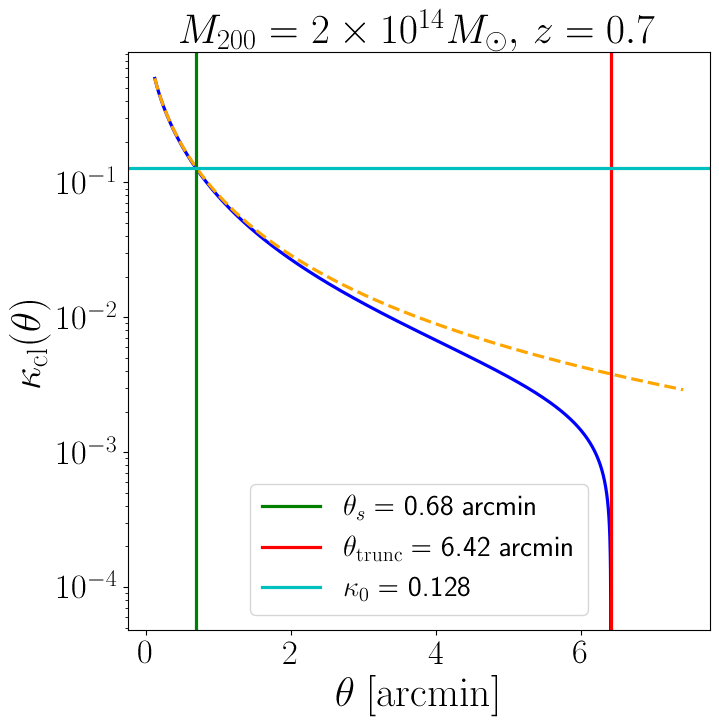
\includegraphics[width=0.7\hsize]{Figures/template_func_theta_.png}}
%     %\subfigure[ ]{
%     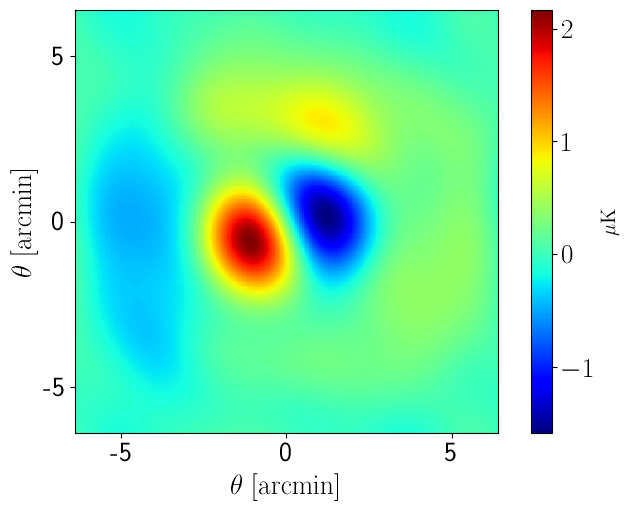
\includegraphics[width=0.85\hsize]{Figures/cluster_dipole.png}%}
%     \caption{The well-known dipole-like structure that we expect in (lensed-unlensed)~\protect\footnotemark[1] sky when there is a cluster with $M_{200} = 2\times 10^{14} M_{\odot}$\protect\footnotemark[2], $z=0.7$ present in our line of sight.}
%     \label{fig:dipole} 
%  \end{figure}
 


\section{Cluster mass estimators}
\label{sec:method}
We describe in \ref{sec:estimators} the MAP reconstruction methodology. We follow  Ref.~\cite{Carron:2017mqf} very closely, but had to adapt some details to make the algorithm work reliably at high resolution and high multipoles in the presence of clusters.
In \ref{sec:cluster_mass} we describe the simple matched filter we use to recover the mass of the cluster from the MAP lensing maps.

\subsection{Lensing Reconstruction}
\label{sec:estimators}
% The most conventional lensing estimate present in the literature is the quadratic estimator \cite{Hu:2001tn, Hu:2001kj, Okamoto:2003zw}. The weak lensing phenomena breaks the statistical isotropic nature of the primordial CMB fluctuations and couples different multipoles in the Fourier space. 
% The quadratic estimator basically uses this strength of coupling in the observed CMB temperature of polarisation maps to estimate the lensing potential or convergence. At the current noise level, the quadratic estimators are nearly fine. In light of future experiments, such as CMB-S4 \cite{CMB-S4:2016ple, CMB-S4:2022ght}, where temperature noise level is as low as 1 $\mu$K-arcmin and polarisation noise level is 1.4 $\mu$K-arcmin, the quadratic estimators are sub-optimal, as the lensing B modes kicks in. 


We work in the flat sky approximation, and identify multipoles to the plane wave vectors $\vell = (\ell_x, \ell_y)$.
% We write the Fourier transform with the compact notation $x(\vell) = \mathcal{Y} x(\vn)$.
As standard in literature, we use $\vell$ for the CMB multipoles and $\vL$ for the lensing multipoles.   

Let $X$ be the unlensed CMB temperature or polarisation field, $X \in \{T, E, B\}$, expressed in Fourier space.
The covariance of these unlensed fields are the primordial power spectra 
$\left<X_{\vell}, X_{\vell'}^\dagger \right> = \delta^{\ell}_{\ell'} C_\ell^{\rm unl}$.

The observed CMB field in pixel space can be expressed as 
\begin{equation}
    X^{\rm dat} = BDX + n
\end{equation}
where $D$ is the operator that maps the unlensed CMB modes to the lensed CMB in real space (and thus contains the Fourier transform operation). The operator $B$ is the linear response matrix of the instrument, including beam and pixel window functions, and $n$ is an independent noise, expressed in pixel space.
When considering the temperature estimator, we have $ X^{\rm dat} = T$, polarization only estimators have $ X^{\rm dat} = (E, B)$, while the minimum variance estimators have  $X^{\rm dat} = (T, E, B)$.

For a fixed deflection field the covariance of the observed CMB fields is
\begin{equation}
    \Cov_{\valpha} \equiv \left<X^{\rm dat} X^{\rm dat, \dagger} \right>_{\valpha}  = BDC^{\rm unl} D^\dagger B^\dagger + N \, ,
\end{equation}
where $N$ is the noise covariance matrix in pixel space. 
While if averaging on the deflection fields as well we can write this covariance as 
\begin{equation}
    \Cov \equiv \left<X^{\rm dat} X^{\rm dat, \dagger} \right> = B \mathcal{Y} C^{\rm len} \mathcal{Y}^\dagger B^\dagger + N \, ,
\end{equation}
where $C^{\rm len}$ is the covariance of the lensed CMB fields, given by the fiducial lensed CMB power spectra, and $\mathcal{Y}$ is the Fourier transform operator.

In pixel space, the unnormalized quadratic estimator of the lensing deflection field can be expressed as the product of two filtered CMB maps
\begin{equation}\label{Eq:QE}
    \hat \valpha^{\rm QE}(\vn) = \bar X(\vn) \, \grad X^{\rm WF}(\vn) \, ,
\end{equation}
where the inverse variance filtered and Wiener filtered legs are
\begin{equation}
    \begin{split}
        \bar X &= B^{\dagger} \Cov^{-1} X^{\rm dat} \, , \\
        X^{\rm WF} &= C^{\rm len}  \mathcal{Y}^\dagger B^{\dagger} \Cov^{-1} X^{\rm dat} \, .
    \end{split}
\end{equation}
The normalisation of the QE is chosen to obtain an unbiased estimator, and is expressed in Fourier space as the isotropic response function $\mathcal R^{\rm QE}(L)$~\cite{Hu:2001kj}.
This gives the normalised QE convergence field in Fourier space
\begin{equation}
    \hat \kappa^{\rm QE}(\vL) = \frac{2}{L^2} \frac{\hat \valpha^{\rm QE}(\vL)}{\mathcal R^{\rm QE}(L)} \,  \, .
\end{equation}

The maximum a posteriori estimator finds the deflection field that maximize the likelihood of the lensed CMB fields, assuming a Gaussian prior on the lensing potential, with power spectrum $C_L^{\phi\phi, \rm fid}$
\begin{equation}
    \ln \mathcal{P}(\valpha | X^{\rm dat}) = \ln \mathcal{L}( X^{\rm dat} | \valpha) - \frac{1}{2} \, \sum_\vL \frac{\left|\phi(\vL)\right|^2}{C_L^{\phi\phi, \rm fid}}
\end{equation}
where the lensed CMB likelihood is assumed to be Gaussian and given by 
\begin{equation}\label{eq:loglik}
    \ln \mathcal{L}( X^{\rm dat} | \valpha) = -\frac{1}{2} X^{\rm dat, \dagger }\Cov_\valpha^{-1} X^{\rm dat} - \frac{1}{2}\ln \det \Cov_\valpha
\end{equation}
In practice, the MAP lensing deflection field $\hat \valpha^{\rm MAP}$ is found by Newton-Raphson iterations on the posterior, starting from $\hat \valpha^{\rm QE}$ until convergence, using the gradient of Eq.~\eqref{eq:loglik} (with respect to the $\valpha$) as search direction. The main term of the gradient can be obtained exactly by running a QE with modified weights on partially delensed CMB maps  \cite[see][for more details]{Carron:2017mqf}. This is the gradient of the first term on the right-hand side in \eqref{eq:loglik}, quadratic in the data for fixed $\valpha$, whose role is to capture the residual lensing signal. The gradient of the second term on the right-hand side, independent of the data for fixed $\valpha$, is the `mean-field', that removes from the quadratic piece signature of anisotropies unrelated to lensing. In our analysis, there is no masking and the noise is statistically isotropic, making the the traditional main sources of mean-field vanish. In principle there is a noise contribution during the iterative procedure: the delensed data noise during the iterative process is not isotropic anymore, because at each step the data is delensed to reduce the CMB anisotropy. This compresses or dilates regions of the sky according to the local estimate of the convergence field, changing the local effective noise levels. This contribution is small and localized at large lensing multipoles, which contributes little to the signal. Hence we neglect the mean field altogether in this paper. 

Unfortunately, the normalization of this estimator is not tractable analytically. We follow \cite{Legrand:2021qdu,Legrand:2023jne} and obtain an empirical normalization of our MAP estimator from a set of simulations.
We generate 1000 CMB flat sky patches, and lens them with random realizations of the large scale structures deflection field. Note that in these simulations we do not include any cluster signal. The empirical normalization is assumed to be isotropic, and is obtained from the cross correlation between the reconstructed $\hat \phi^{\rm MAP}$ and the input lensing potential $\phi^{\rm in}$, averaged over our set of simulations
\begin{equation}
    \mathcal{W}^{\rm MAP}_L = \left< \frac{C_L^{\phi^{\rm in}, \hat \phi^{\rm MAP}}}{C_L^{\phi^{\rm in}, \phi^{\rm in}}} \right> \; .
\end{equation}
As shown in \cite{Legrand:2021qdu,Legrand:2023jne}, this empirical normalization is not sensitive to the cosmology, input lensing or data noise, allowing for a correct normalization also when the fiducial ingredients entering the reconstruction process are a poor match to those of the data.


In the posterior maximization process, delensing of the CMB occurs via the operator $D^\dagger$. Our first implementations of the MAP solver in Ref.~\cite{Carron:2017mqf} made the additional assumption of the invertibility of the deflection field, and performed remappings of the maps using a standard bicubic spline algorithm. To improve stability and performance, we updated our flat-sky tools with the lensing method of Ref.~\cite{Reinecke:2023gtp}, based on non-uniform FFTs techniques~\cite{Barnett2019, Barnett2020}. This method is extremely accurate and at the same time removes this unnecessary assumption of an invertible deflection. With this, we found that the search for the MAP point converges without issues on all relevant scales, after only 10-20 iterations\JC{is that right ?} \bb{yes}.


\subsection{Cluster Signal Reconstruction}
\label{sec:cluster_mass}
\LL{Should add a comment that to have the template kt we first need an estimate of the angular size of the cluster $\theta_s$ (which can be obtained from SZ effect like in Zubeldia paper, or else)}
\bb{Yes you are right! $\theta_s$ estimate comes from empirical form of $c_{200}$ which has been mensioned and referred in Eq.~\ref{eq:c200}.} \LL{But we dont know M200 before, so how do we get the template in the first place?}

Once we have reconstructed the lensing map $\hat{\kappa} (\vL)$ from the simulated CMB data, we fit our theoretical template $\kappa_0\kappa^t (\vL)$. We do this assuming an isotropic Gaussian noise spectrum $N(\vL)$, such that $\langle{\hat{\kappa} (\vL) \hat{\kappa} (\vL')}\rangle - \langle{\hat{\kappa} (\vL)}\rangle \langle \hat{\kappa} (\vL') \rangle = \delta(\vL - \vL') N (\vL)$. This allows us to construct a minimum variance estimator for $\kappa_0$, given by
\begin{equation}\label{eq:kappa_0}
    \hat{\kappa}_0 = \frac{ \displaystyle \int \frac{\diff^2\vL}{(2\pi)^2} \frac{\kappa_t(\vL) \hat \kappa(\vL)}{N(\vL)}}{\displaystyle  \int\frac{\diff^2\vL}{(2\pi)^2} \frac{|\kappa_t(\vL)|^2}{N(\vL)}}.
\end{equation}
Owing to spherical symmetry, all quantities but $\hat{\kappa} (\vL)$ in the aforementioned expression are functions of $L = |\vL|$ \LL{It is an approximation for N(L), see my comment below}. The theoretical error $\sigma^{2,\rm th}_{\kappa_0}$ for the estimator is as follows:
\begin{equation}\label{eq:kappa_0_noise}
\frac{1}{\sigma^{2,\text{th}}_{\kappa_0}} = \frac{1}{2\pi}\int_{L_{\rm min}}^{L_{\rm max}} dL L \frac{|\kappa_t(L)|^2}{N(L)},
\end{equation}
for which we often use the curved-sky expression
\begin{equation}
\frac{1}{\sigma^{2,\text{th}}_{\kappa_0}}=	\sum_{L=L_{\rm min}}^{L_{\rm max}} \left( \frac{2L + 1}{4\pi} \right)\frac{|\kappa_{t,L}|^2}{N_L}
\end{equation}
In these equations, the noise of the $\hat \kappa(\vL)$ estimate is given by \begin{equation}\label{eq:Noisespec}
 	N_L = C_L^{\kappa\kappa} + N_L^{(0)} + N_L^{(1)},
 \end{equation}
where $C_L^{\kappa\kappa}$ is the power spectrum of the background convergence profile of the large-scale structure exclusive of the cluster, which contributes to the Gaussian noise on the cluster lensing signal. In the case that $\hat \kappa$ is the QE estimate, $N^{(0)}_L$ is the leading CMB-lensing reconstruction noise (the disconnected four-point function), and $N^{(1)}_L$ the connected part originating from the secondary trispectrum contractions, proportional to $C_L^{\kappa\kappa}$~\cite{Kesden:2003cc,Lewis:2006fu}. In the MAP case, the same Eq.~\eqref{eq:Noisespec} provides a good fit to the spectrum, with both noise terms calculated with partially delensed spectra, following Ref.~\cite{Legrand:2021qdu}. On hypothetical maps where the cluster lensing signal were the only lensing-like signal, only $N^{(0)}_L$ would be present.\JC{How much of a difference would it make, could we just quote quickly a number?}

\LL{At the small scales, the assumption of Eqs.~\ref{eq:kappa_0_noise} and \ref{eq:Noisespec} that the noise covariance $N(\vL, \vL')$ is diagonal breaks down: the non diagonal terms can be of the same order as the diagonal ones. This can be interpreted as a tight correlation between modes that share the same large scale gradient \cite{Horowitz:2017iql}. The diagonal assumption of Eq.~\ref{eq:kappa_0_noise} then leads to an underestimate of the variance of $\hat \kappa_0$. This is particularly true for the QE. For the MAP, Ref.~\cite{Legrand:2021qdu}}\JC{slightly confused here by this discssion, spectrum covariance or map covariance?} \LL{showed that the covariance matrix is well approximated by diagonal, so Eq.~\ref{eq:kappa_0_noise} is a better approximation.}


\LL{Impact of the miscentering?}
\bb{We haven't discussed it. tbh, I don't know as well.}


In Figure~\ref{fig:int}, we show the contribution of each lensing multipole to the theoretical signal to noise of Eq.~\ref{eq:kappa_0_noise}. These curves are obtained with the theoretical $N_L^0$ and $N_L^1$ of each estimator, considering a  CMB-S4 like experiment with white noise level of $1 \mu \rm{K}$-arcmin in temperature and $\sqrt{2} \mu K$-arcmin in polarization and a beam full width at half-maximum (FWHM) of 1 arcmin. 
We considered a cluster of mass of $M_{200} = 2\times 10^{14}$, at $z=0.7$, which reflects roughly the expected mean mass and redshift of the CMB-S4 clusters detected with thermal SZ effect \cite{CMB-S4:2016ple}. 

We include multipoles $\ell_{\text{min}}^{\, \text{CMB}} = 100$ to $\ell_{\text{max}}^{\, \text{CMB}} = 4000$ of the CMB temperature and polarization maps for the lensing reconstruction. 
We compare both the QE and the MAP estimators. We also show the modified QE noted HDV \cite{Hu:2007bt} with a scale cut on the gradient leg of temperature map at $\ell_{\rm cut}=2000$ \LL{correct?}, which is introduced in more details below. 

We see that for both QE and MAP, the lensing scales that dominates the signal to noise are around $L\sim 2000$ in the temperature and around  $L\sim 1100$ in the polarization. The HDV estimator mainly loose information on the large scales, for $L \lesssim 2000$, while smaller scales contain similar information as compared to the QE.
This shows that for this CMB-S4 configuration and cluster convergence profile, temperature and polarization channels are bringing similar level of information, albeit from different scales.  
Finally we clearly see that the MAP estimator outperforms the QE at all lensing scales, and this improvement is mainly due to increased signal from the polarization channel. 

\begin{figure}
    \centering
    \hspace*{-1.0cm} 
    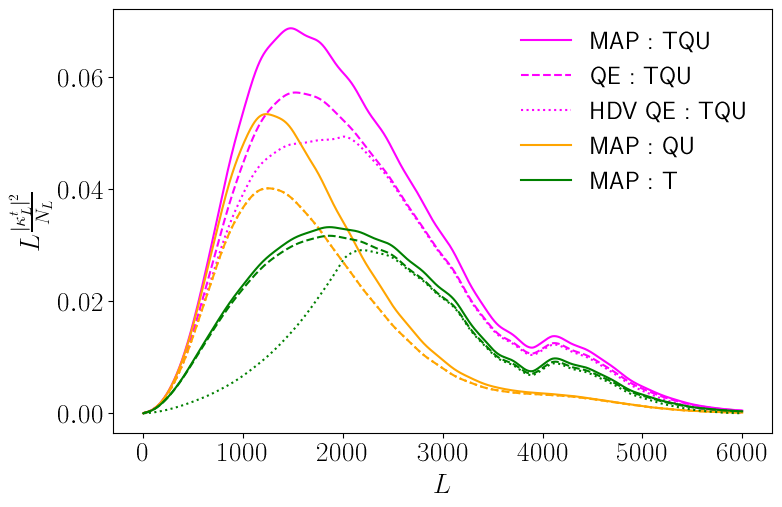
\includegraphics[width=1.\hsize]{Figures/Integrand.png}
    \caption{Contribution per lensing multipole to the cluster mass SNR (the integrand of Eq.~\ref{eq:kappa_0_noise}). Green, blue and pink show temperature-only, polarization-only and combined reconstruction respectively. Solid show the quadratic estimator case and dashed the CMB lensing maximum a posteriori method of this work\JC{Fixed solid vs dashed, HDV description missing}. Shown is the case of a $2\cdot 10^{14} M_\odot$ cluster at $z = 0.7$, for the CMB-S4-like configuration given in the text. While the MAP approach is exactly the same than for optimal CMB lensing power spectrum reconstruction, this is probing much smaller scales (the spectrum SNR is almost entirely confined to $L < 1500$ for this configuration).}
    \label{fig:int}
\end{figure}

\section{Results}
\label{sec:results}

In this section, we present results on the cluster convergence profile and on the cluster mass from reconstructions of the lensing signal from a set of simulations. 
Our simulations reproduce a CMB S4-like experiment \cite{CMB-S4:2016ple}, with white noise level is  $1 \mu \rm{K}$-arcmin in temperature and $\sqrt{2} \mu \rm{K}$-arcmin in polarization. We assume a beam with a full width at half-maximum (FWHM) of 1 arcmin. 
Our flat sky patches have a pixel size of $0.3$ arcmin with 1024 pixels on a side. We simulate the lensing by both the large scale structures and the dark matter halo, assuming they are uncorrelated. The dark matter haloes are centered on the patches. 
% In our baseline analysis, we simulate a halo mass $M_{200} = 2\times10^{14} M_{\odot}$ with $z=0.7$. 

We test both the quadratic estimator and the MAP estimator, as introduced in Section~\ref{sec:estimators}, to obtain the estimated $\hat{\kappa}(L)$.
We then estimate the mass of the cluster with the matched filtering, as described in Section~\ref{sec:cluster_mass}. We compare our results for the temperature only (T), the polarization only (QU) and the minimum variance (MV) estimators.

% by Eq. \ref{eq:ft_anal1} and \ref{eq:ft_anal2} \LL{its not in Eq \ref{eq:kappa_0} ?}.
% To simplify the calculations, we employ the flat-sky approximation.
% In the first part of this section, we examine the low bias in temperature caused by moderate to strong lensing in the cluster center. In the second part, we present the results of our estimator, along with the corresponding theoretical forecast, assuming that $M_{200}$ is $2\times10^{14} M_{\odot}$ and $z$ is $0.7$.

\subsection{Bias in Temperature QE}

\begin{figure*}
    \subfigure[ ]{
    \label{fig:kappa_th}
    \hspace*{-1.0cm}
    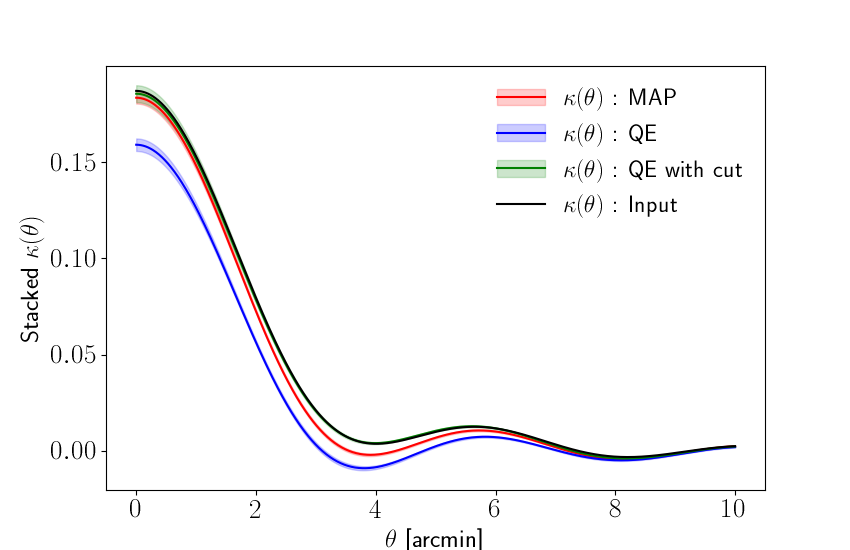
\includegraphics[width=0.55\hsize]{Figures/kappa_thet_lmax5k_out5k_M4.png}}
    \subfigure[ ]{
     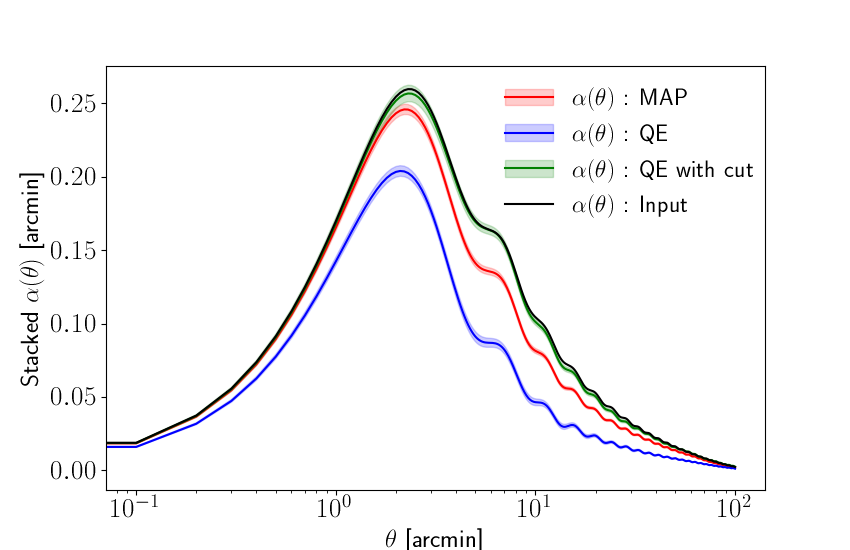
\includegraphics[width=0.55\hsize]{Figures/alpha_thet_lmax5k_out5k_M4.png}}
  \caption{Reconstructed convergence (left) and deflection angle $\alpha$ (right) profiles from  stacking a set of $1000$ temperature-only reconstructions ($M = 4 \cdot 10^{14} M_\odot, z=0.7$). CMB multipoles $100 \leq \ell \leq 5000$ are used to reconstruct the lensing multipoles $100 \leq L \leq 5000$. Shown are the standard QE (blue), QE with a high-$\ell$ cut at $2000$ on the gradient leg~\cite{Hu:2007bt}(green), and the maximum a posteriori (MAP) lensing reconstruction of this work (red, without any cuts), and the input truncated to the same $L$ range. The bias in the MAP reconstruction is much reduced compared to the QE but still visible at this cluster mass. In polarization reconstruction no such bias is visible in either case.}
  \label{fig:Bias_sup}
  \end{figure*}

As discussed in the literature \cite{Maturi:2004zj, Hu:2007bt} the temperature QE is biased low due to strong to moderate lensing close to the cluster center. 
As lensing by the cluster magnifies the background CMB, the gradient of the observed CMB is smaller than the unlensed CMB gradient.
Since the weak lensing signature, i.e. the dipole-like structure in the lensed-unlensed sky, is sensitive to both the strength of the gradient and the mass of the cluster, it decreases that signature as well. 
As a consequence, when we estimate cluster signal using weak lensing temperature QE, the estimator is biased low.

The temperature quadratic estimator is nothing but a product of two filtered maps as given in Eq.~\ref{Eq:QE}. The bias comes mainly from the small scales in the gradient leg. 
A solution to this bias, as demonstrated in \cite{Hu:2007bt}, is to use a low-pass filter for the gradient leg and only include multipoles below $\ell=2000$. We denote as HDV this modified QE with a scale cut.
% In Appendix~\ref{A1}, we present the analytical forecast on the performance of such modified QE compared to conventional QE in the context of the bias\JC{??}.


Since the bias is more prominent for massive clusters and small scales, we choose here the clusters parameters to be $M_{200} = 4 \times 10^{14} M_{\odot}, z=0.7$ and use CMB multipoles from $\ell_{\text{min}}^{\, \text{CMB}}=100$ to $\ell_{\text{max}}^{\, \text{CMB}} = 5000$. 
We run all the estimators (QE, HDV and MAP) with the temperature only channel, on $1000$ simulations, and stack the reconstructed maps.
We also subtract the noise of the reconstruction to eliminate the variance of the noise due to stacking. \LL{how do you estimate the noise?}

In Figure~\ref{fig:Bias_sup}, we provide the comparison for the deflection profile, $\alpha(\theta)$  and the convergence profile $\kappa (\theta)$. 
Although, $\alpha$ and $\kappa$ are reconstructed in 2D patch, we bin the polar angle to get an one dimensional plot as a function of radius (or angular distance from the centre) of those quantity. 
The deflection $\alpha$, which is the gradient of the lensing potential $\phi$ is a vector quantity. 
But only its radial component is expected to be non-zero, since cluster is circularly symmetric. 
Hence we only binned radial component of $\alpha$. As expected the QE is biased low for such massive clusters, whereas the modified QE~\cite{Hu:2007bt} with the cut in the gradient leg does almost unbiased reconstruction of the cluster signal. 
Our iterative estimator in other hand, does manage to get rid of the bias up to some limit\JC{Must quantify this}, without wasting any information in the small scale regime\JC{how much was wasted with cut?}.
Therefore, in the next section, we discuss how the iterative estimator also suppresses the noise of the mass estimation compared to QE. We refer to the modified QE as QE \JC{hmm} for the temperature estimator from now on.


% We show in Fig.~\ref{fig:Bias_sup} the reconstructed convergence profiles for the QE and MAP estimators, from our set of simulations at redshift xxx and mass xxx \LL{Sayan maybe here you can comment more the plots.}.


\subsection{Cluster mass constraints}

\begin{table}
\centering
\hspace*{1.0cm} 
\caption{\textbf{Summary of results on 1000 simulations with Input $\bs{\kappa_0 = 0.1285}$}\JC{Description missing. Fix notation of theoretical error in 3.11}}
    \begin{tabularx}{0.15\textwidth}{|X|X|}
    \hline
    \multicolumn{2}{|c|}{QE : T} \\ \hline
    $\langle\kappa_0 \rangle$      & 0.1275   \\ \hline
    $\sigma_{\kappa 0}$ & 0.0099  \\\hline
    $\sigma_{\kappa 0}^{\text{th}}$ & 0.0096  \\\hline
    \end{tabularx}
    \begin{tabularx}{0.15\textwidth}{|X|X|}
    \hline
    \multicolumn{2}{|c|}{QE : QU} \\ \hline
    $\langle\kappa_0 \rangle$      & 0.1397   \\ \hline
    $\sigma_{\kappa 0}$ & 0.0088  \\\hline
    $\sigma_{\kappa 0}^{\text{th}}$ & 0.0090  \\\hline
    \end{tabularx}
    \begin{tabularx}{0.15\textwidth}{|X|X|}
    \hline
    \multicolumn{2}{|c|}{QE : TQU} \\ \hline
    $\langle\kappa_0 \rangle$      & 0.1309   \\ \hline
    $\sigma_{\kappa 0}$ & 0.0064  \\\hline
    $\sigma_{\kappa 0}^{\text{th}}$ & 0.0067  \\\hline
    \end{tabularx} \\ 
    \begin{tabularx}{0.15\textwidth}{|X|X|}
    \hline
    \multicolumn{2}{|c|}{MAP : T} \\ \hline
    $\langle\kappa_0 \rangle$      & 0.1272   \\ \hline
    $\sigma_{\kappa 0}$ & 0.0082  \\\hline
    $\sigma_{\kappa 0}^{\text{th}}$ & 0.0083  \\\hline
    \end{tabularx}
    \begin{tabularx}{0.15\textwidth}{|X|X|}
    \hline
    \multicolumn{2}{|c|}{MAP : QU} \\ \hline
    $\langle\kappa_0 \rangle$      & 0.1342   \\ \hline
    $\sigma_{\kappa 0}$ & 0.0078  \\\hline
    $\sigma_{\kappa 0}^{\text{th}}$ & 0.0081  \\\hline
    \end{tabularx}
    \begin{tabularx}{0.15\textwidth}{|X|X|}
    \hline
    \multicolumn{2}{|c|}{MAP : TQU} \\ \hline
    $\langle\kappa_0 \rangle$      & 0.1331   \\ \hline
    $\sigma_{\kappa 0}$ & 0.0061  \\\hline
    $\sigma_{\kappa 0}^{\text{th}}$ & 0.0062  \\\hline
    \end{tabularx}
    \label{tab:results}
\end{table}

We now consider 1000 simulations with a cluster mass of $M_{200} = 2 \times 10^{14} M_{\odot}$ and $z=0.7$, closer to the expected mean mass of the CMB-S4 clusters. We reconstruct the lensing signal with scales between  $\ell_{\text{min}}^{\, \text{CMB}}=100$ and $\ell_{\text{max}}^{\, \text{CMB}} = 4000$ \LL{to check}, for both polarization and temperature maps.
We reconstruct the lensing convergence fields with the three estimators: QE, HDV and MAP, and with the temperature only (T), polarization only (QU) and minimum variance (MV) estimators. We then run a matched filter on these reconstructed lensing map to estimate the convergence amplitude $\hat \kappa_0$, assuming a template $\kappa_t$ with the characteristic angular size $\theta_s$ corresponding to the input mass and redshift of the cluster profiles. 
We use the lensing multipoles beateen $L_{\text{min}}=100$ and $L_{\text{max}}=6000$ to obtain $\hat \kappa_0$ from Eq.~\ref{eq:kappa_0}. We compute the variance of $\hat \kappa_0$ from our set of 1000 simulations, and compare to the theortical expectations of the variance from Eq.~\ref{eq:kappa_0_noise}.
Table~\ref{tab:results} summarizes our results. 
We see that as expected, the standard QE is biased low $\kappa_0$ in temperature, and that the HDV greatly reduce this bias. 
The MAP estimator however is unbiased (?)
Constraints with the MAP are increased by xx\% compared to the HDV
\LL{to develop given the last version of the Table}. \LL{Give bias in terms of number of sigma}. 


In Figure~\ref{fig:forecast} we show the theoretical relative error on the mass for a set of 1000 clusters. We compare our set of estimators for different white noise level of the CMB experiment. As illustration we plot the standard deviation we recovered from our simulations.  We see that for the CMB-S4 noise level, simulations perform as expectations. Moreover, we see that the MAP estimator allows to recover the loss in constraining power from the HDV estimator. Finally, it is clear that as we go to lower noise level, the polarization estimator will totally dominate the constraints. 

% In Table~\ref{tab:results}, we provide the summary of our results using the estimators on simulations along with the forecast on noise for those estimator, using use $L_{\text{min}}=100$ and $L_{\text{max}}=6000$. We also plot those results along with the forecast of mass estimation in Figure~\ref{fig:forecast}.   \JC{Description of the results?}
\begin{figure}
    \centering
    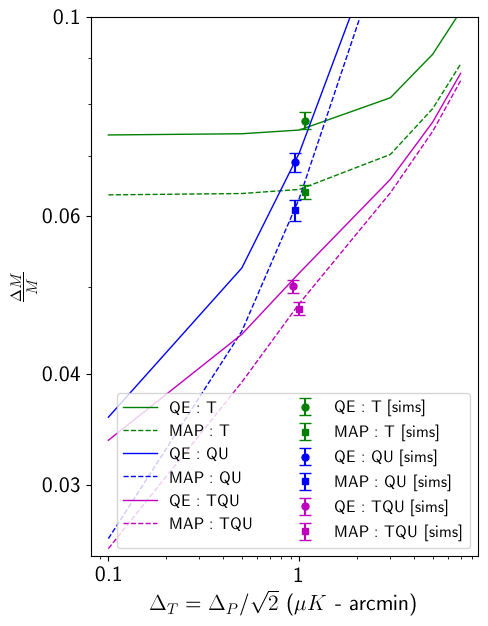
\includegraphics[width=1.\hsize]{Figures/forcast_snr.png}
    \caption{Constraints on cluster mass for a sample of 1000 identical clusters ($M_{200} = 2\times10^{14}M_{\odot}$, at redshift 0.7) as a function of white noise levels. The beam FWHM is $1$ arcmin.\JC{HDV stands for the QE with a cut at $2000$ in the gradient leg~\cite{Hu:2007bt} to remove the QE bias (see Fig.~\ref{fig:Bias_sup} FIX fig ref}. The improvement in constraint \JC{from the dashed to solid ?} comes from the partial removal from the CMB map of the lensing signal unrelated to the cluster, and is more prominent in polarization, as expected. The error bars indicate results obtained from 1000 simulations, showing consistency.}
    \label{fig:forecast}
\end{figure}


\LL{Should compare these results with Srini paper \cite{Raghunathan:2017cle}}

\JC{The remainder of this section needs rewriting}
As mentioned in the previous section, we employ the modified QE~\cite{Hu:2007bt} for the temperature estimator, referred to as `QE : T' in this section. 
With the noise level of the CMB S4, the MAP estimator detects the cluster signal with a significance of $21.8\sigma$, representing an approximate $5\%$ \JC{?? how was this calculated ?}enhancement compared to QE.
While our results are presented based on 1000 simulations, they can be extrapolated to the projected number of clusters in CMB S4, estimated to be $10^5$. 
In our analytical forecasts and the estimation on simulations, we have included the lensing of CMB from the large scale structure (LSS) as well. 
In the context of cluster-lensing, it is accounted as a Gaussian noise. 
Although the LSS-lensing is supposed to vanish due to stacking of sky-patches, it still contributes to the noise of lensing reconstruction. 
Hence, it is important to account for the LSS lensing and all the complicacy that comes with it. 
It is worth noting that in both our analytical forecasts and simulations, we accounted for the lensing effects of the large-scale structure (LSS) on the CMB. 
In the realm of cluster-lensing, the LSS lensing is treated as Gaussian noise. 
Despite efforts to mitigate its impact through stacking of sky-patches, the LSS lensing still contributes to the noise in the lensing reconstruction process. 
Thus, it is crucial to consider the influence of LSS lensing and all the associated complexities it brings.
%We expect $10^5$ number of clusters to be detected for S4 experiment. We provide the forecast on Inverse signal to noise ratio (SNR) for $10^5$ for conventional QE and MAP estimator in figure and we show the improvement in figure . We consider modes from $\ell_{min}=100$ to $\ell_{max}=4000$ in the lensed CMB maps for estimating $\hat \kappa (\ell)$ in both cases.

%\begin{figure}[H]
%   \centering
%   \subfigure[ ]{
%   \label{fig:snr_4k}
   %\hspace*{-1.4cm}
%   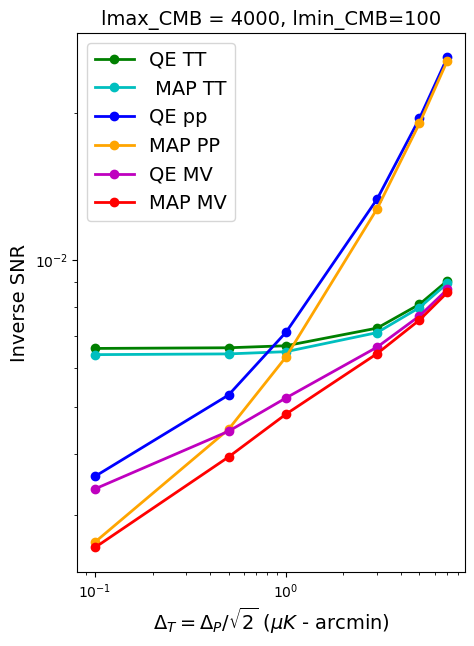
\includegraphics[width=0.7\hsize]{Figures/snr_forecast_lmax4k.png}}
%   \subfigure[ ]{
%   \label{fig:improvement}
%   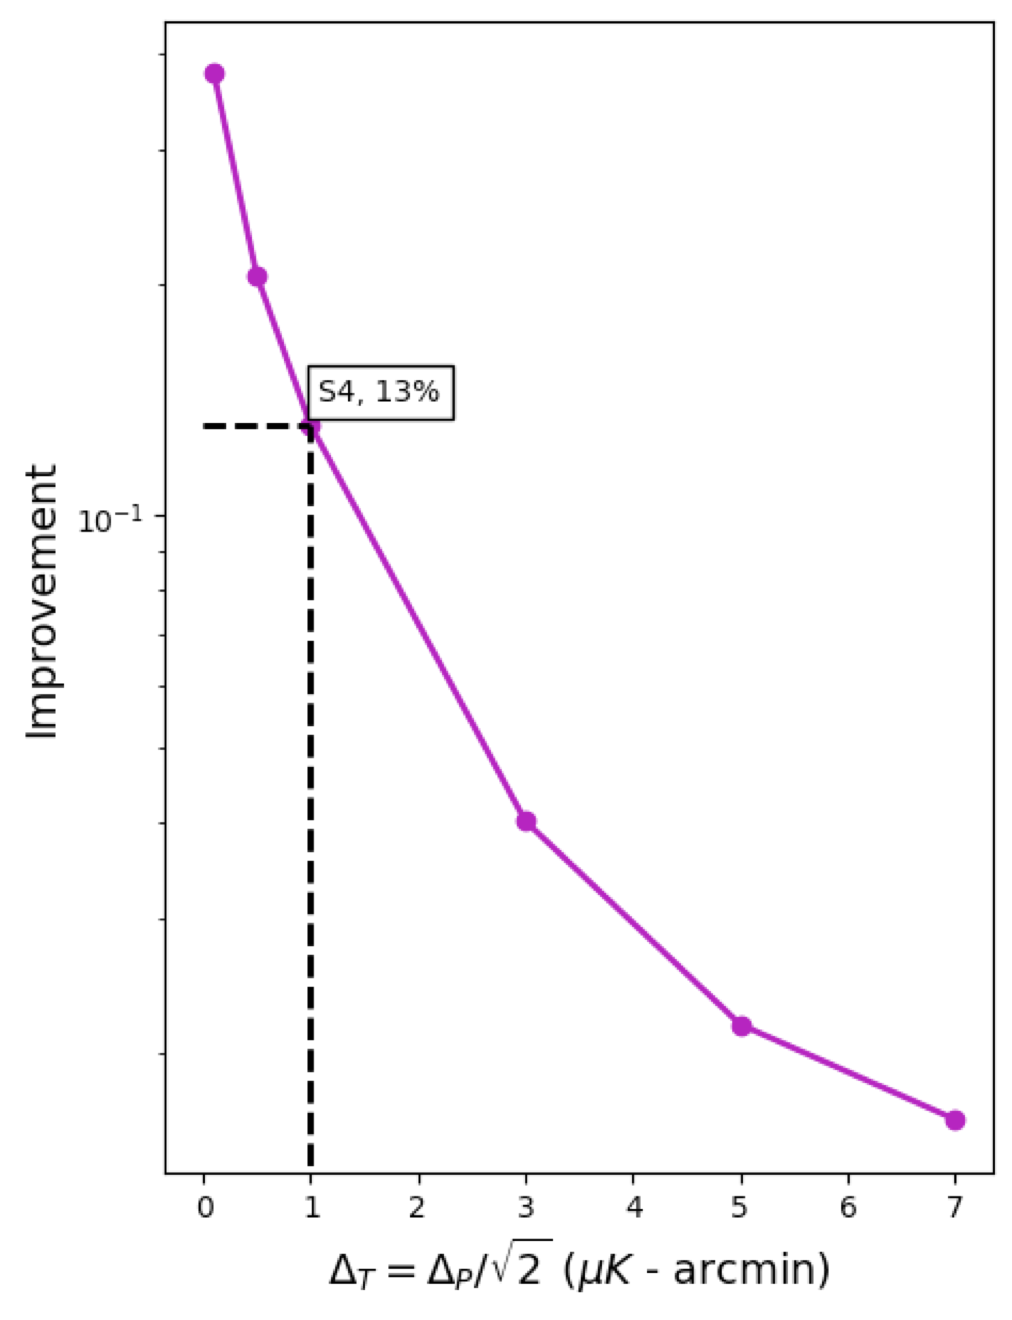
\includegraphics[width=0.7\hsize]{Figures/improvement_lmax4k.png}}
%   \caption{}
%\end{figure} 

\section{Conclusions}
\label{sec:conclusion}

\LL{tentative conclusion}
In this work we demonstrated the use of the maximum a posteriori estimator to reconstruct the mass profile of galaxy clusters. We showed that the constraints on the cluster reach the forecasted ones.
The MAP estimator improves the constraints on the cluster mass by a factor \LL{xxxx} compared to the HDV QE \cite{Hu:2007bt}

The MAP estimator does not suffer from the bias of the QE, arising from the misestimate of the background gradient CMB modes. This can be interpreted by the fact that the MAP estimate the delensed CMB modes, and as such gets more accurately the unlensed large scale gradient. 
This permits the use of all CMB scales in the reconstruction, without the necessity of scale cuts as in \cite{Hu:2007bt}. 

The MAP reconstruction algorithm received considerable increase in the speed and accuracy of the lensing/delensing operations, lowering its numerical cost \cite{Reinecke:2023gtp}. The MAP estimator cost is for instance much lower than the maximum likelihood estimator which requires of order $10^5$ simulations per redshift and mass \cite{Raghunathan:2017cle}. 

Our simulations went a step further than most current analyses by including the lensing from the background large scale structures together with the cluster. \LL{this increase the variance of the QE, but is negligible for the MAP??}. We however assumed that the background LSS are independent from the cluster. In reality, clusters are located at the nodes of the cosmic web, and are highly correlated with overdensity regions. Dark matter simulations such as the Websky \cite{Stein:2020its} and DEMNUni \cite{Carbone:2016nzj} should be used to evaluate this impact. 

Some other caveats still remain. We did not consider the contaminations from foregrounds signal, such as the SZ effect, radio point sources or the Cosmic Infrared Background. The thermal SZ effect has a frequency dependance which allows to remove its contribution from the observed CMB maps, at the expense of increased variance. It is possible to reduce the loss of signal in the lensing reconstruction by tSZ cleaning only the gradient leg of the QE \cite{Madhavacheril:2018bxi, DES:2018myw, Patil_2020}. The kinematic SZ however cannot be distinguished from the lensing signal. A more careful analysis of the MAP reconstruction should include these contaminating signals. However, it is expected that the polarization foregrounds are negligible at the small scales, so our MAP estimator forecast in polarization should in principle stay accurate. 

The normalization of the MAP estimator requires careful handling. Indeed it cannot be obtained analytically and we relied on a set of fiducial simulations to obtain it. In the context of the large scale structures, we showed in \cite{Legrand:2021qdu} that this normalization is independent of the true cosmology and noise level of the CMB.  \LL{Do we expect more problems with the normalisation for cluster lensing, like MF or else?}

\JC{Work is needed in this section}
In this study, we have conducted an investigation into the phenomenon of CMB lensing by galaxy clusters, with a particular focus on utilizing this process to reconstruct the mass profile of the clusters. To address the inherent challenges associated with this task, we have introduced the maximum a posteriori (MAP) estimator~\cite{Carron:2017mqf} as a novel approach for accurately estimating the convergence $\kappa$ in the context of cluster lensing.

A primary concern we have addressed pertains to the bias observed in the temperature quadratic estimator (QE) when strong to moderate lensing occurs near the central region of the cluster. While the modified QE successfully mitigates this bias, it introduces additional noise due to the underutilization of information at small scales. Conversely, our findings indicate that the MAP estimator offers improved performance over the QE approach by effectively reducing the bias without compromising information extraction at small scales. Consequently, the MAP estimator emerges as an appealing choice for the task of reconstructing cluster masses.

In the subsequent section of our study, we have quantitatively assessed the performance of the MAP estimator in the presence of CMB S4 noise. By considering a sample size of $1000$ clusters, we report a highly significant detection of the cluster signal with the MAP estimator, reaching a level of $21.8\sigma$. Notably, this represents an approximate $5\%$ improvement in detection significance compared to the QE approach. These outcomes underscore the robustness and precision of the MAP estimator in the realistic observational context of cluster signal detection.

In summary, our study demonstrates the efficacy of the MAP estimator in mitigating bias and enhancing the accuracy of mass estimation in the realm of cluster lensing. Through a rigorous comparison with the QE approach, we have substantiated the distinct advantages offered by the MAP estimator in addressing bias while fully utilizing available information. These findings contribute to the advancing body of knowledge concerning CMB cluster lensing and provide valuable insights for future investigations focused on the reconstruction of galaxy cluster mass profiles through the exploitation of CMB lensing techniques.
\JC{mention tough aspects like calculation of WF}

\begin{acknowledgements}
The authors acknowledge helpful discussions with Mathew Madhavacheril and Sebastian Belkner. The computations were performed at University of Geneva on ``Yggdrasil" HPC cluster. SS acknowledges support from the Federal Commission for Scholarships for Foreign Students for the Swiss Government Excellence Scholarship (ESKAS No. 2022.0316) for the academic year 2022-'23. LL and JC acknowledge support from a SNSF Eccellenza Professorial Fellowship (No. 186879).

\end{acknowledgements}
%\onecolumngrid
\bibliography{CL}
\appendix
\section{Theoretical Expressions in Clusters Lensing}\label{A2}
The expression for the convergence profile of the galaxy clusters is given by~\cite{Takada:2002qq},
\begin{equation}
    \kappa_{cl} = \frac{2\rho_s r_s}{\Sigma_{crit}(z)}g(x), \text{ where } x=\frac{r}{r_s} = \frac{\theta}{\theta_s},
\end{equation}
and where $g(x)$ is a circularly symmetric function depending on the truncation of the profile,
\begin{equation}
    g(x) = 
     \begin{cases}
       -\frac{\sqrt{x_{\text{max}}^2-x^2}}{(1-x^2)(1+x_{\text{max}})} + \frac{1}{(1-x^2)^{\frac{3}{2}}}&\cosh^{-1}\left(\frac{x^2+x_{\text{max}}}{x(1+x_{\text{max}})}\right),  \\ &(x < 1)\\
       \frac{\sqrt{x_{\text{max}}^2 - 1}}{3(1+x_{\text{max}})}\left[ 1+\frac{1}{1+x_{\text{max}}} \right],  &(x = 1)\\
       -\frac{\sqrt{x_{\text{max}}^2-x^2}}{(1-x^2)(1+x_{\text{max}})} - \frac{1}{(x^2-1)^{\frac{3}{2}}}&\cosh^{-1}\left(\frac{x^2+x_{\text{max}}}{x(1+x_{\text{max}})}\right),  \\
       &(1< x \leq x_{\text{max}})\\
     \end{cases}
\end{equation}
where we introduced $x_{\text{max}}$, the ratio of the truncation radius to $r_s$, which in our case is equal to $3\times c_{200}$. 
The analytical form of the Fourier transform to the convergence profile, equivalent to Eq.~\ref{eq:FT1} and \ref{eq:FT2}, is given by \cite{Scoccimarro:2000gm, 2011PhRvD..83b3008O, Takada:2002qq}%in Eq 10 of \cite{Scoccimarro:2000gm}, Eq 28, 29 of \cite{2011PhRvD..83b3008O} or Eq 17 of \cite{Takada:2002qq}, but slight modification: $c_{200}$ is replaced by $x_{\text{max}}$, but the normalisation $m_{\text{nfw}}$ is always the same (depends on $c_{200}$ doesn't depend on $R_{\text{trunc}}$) 
\begin{equation}\label{eq:ft_anal1}
    \kappa_{a}(l;z) = \frac{M_{200}\Tilde{u}(k=\ell/\chi;z)}{(1+z)^{-2}\Sigma_{\text{crit}}(z)},
\end{equation}
where $\Tilde{u}(k=\ell/\chi;z)$ is given by
\begin{align}\label{eq:ft_anal2}
    \Tilde{u}(k=\ell/\chi;z) = \frac{1}{m_{\text{nfw}}}[\sin{y}\{\text{Si}[y(1+x_{\text{max}})] -\text{Si}(y)\} \nonumber \\ 
    +\cos{y}\{ \text{Ci}[y(1+x_{\text{max}})]-\text{Ci}(y) \} - \frac{\sin{(y x_{\text{max}})}}{y(1+x_{\text{max}})}].
\end{align}
Here, we define a new Fourier variable, $k =\ell/\chi$. $\chi$ is the comoving angular diameter distance at that redshift, defined as $\chi(z) = \int_0^z dz'\frac{1}{H(z')} = (1+z)d_A(z)$. In the above equation, $y = (1+z)kr_s$; $\text{Si}(x)$ and $\text{Ci}(x)$ are the sine and cosine integrals and the normalisation $m_{\text{nfw}} = \ln{(1+c_{200})}-\left(\frac{c_{200}}{1+c_{200}}\right)$.

%The analytical expression matches with Wigner transform of the profile or Fast Fourier Transform of a 2D circularly symmetric convergence profile. 

%Since the convergence profile is circularly symmetric, we can use standard simplifications in Fourier space, as follows
%\begin{equation}\label{eq:FT1}
%    \kappa(L) = \int d^2 \theta\: \kappa(\theta) e^{- i \bs{L}\cdot\bs{\theta}} = 2\pi \int_0^{\infty} d\theta \: \theta \kappa(\theta) J_0(\theta L)
%\end{equation}
%Here $J_0$'s are first kind Bessel's function of zeroth order. We can use the asymptotic approximation of the Legendre Polynomial, i.e. $P_L(\cos \theta) \underbrace{\rightarrow}_{L \rightarrow \infty} J_0(L \theta)$ to express the above expression as the spin 0 Wigner transform of the convergence profile.
%\begin{equation}\label{eq:FT2}
%    \kappa(L) \sim 2\pi \int_{-1}^1 d \cos (\theta )\:\kappa(\theta) P_L(\cos \theta)
%\end{equation}
%The transform is also circularly symmetric in 2D Fourier space. The analytical form of the Fourier transform has been provided in Appendix~\ref{A2}.


\section{Exact QE average for fixed deflection}\label{A1}
\newcommand{\hn}[0]{\hat n}
In this section we sketch how we obtain the exact expectation value of a quadratic estimator (QE) in the presence of a fixed deflection field. This allows us to predict the mass bias suffered by QE mass estimates.

We consider a generic separable temperature QE, described by two isotropic functions $F_l$ and $G_l$. Following \emph{Planck}-lensing style notation, it may be written in configuration space,
\begin{equation}
	_{1}\hat g(\hat n) = \left( \sum_{l_1m_1} F_{l_1} T_{l_1m_1}\:_sY_{l_1m_1}(\hn) \right) \left( \sum_{l_2m_2} G_{l_1} T_{l_2m_2}\:_tY_{l_2m_2}(\hn) \right) 
\end{equation}
In the case of interest, lensing, we have $s =0, t = 1$, and
\begin{equation}
	F_l = \frac{1}{C_l + N_l}, \quad G_l = - \sqrt{l(l+ 1)}\frac{C_l}{C_l + N_l},
\end{equation}
Here, $_{1} \hat g(\hat n)$ is the unnormalized deflection vector (spin-1) field estimate. We want to evaluate this quantity
\begin{equation} \label{eq:avg}
	\av{\: _{1}\hat g(\hat n)}_{\text{fixed $\phi$}},
\end{equation}
which may be used to predict the result of stacking QEs from CMB maps on identical clusters.

Let $\hat n'$ be the undeflected position that corresponds to the observed location $\hn$. Working at fixed $\hn$, by Fourier transforming the $T$-maps, we may write this as a cross-spectrum,
\begin{equation}\label{eq:g}
\begin{split}
	\av{\: _{1}\hat g(\hat n)}_{\text{fixed $\phi$}}
=\sum_{lm} C_l F^*_{lm}(\hn) G_{lm}(\hn)
 \end{split}
\end{equation}
with 
\begin{equation}
\begin{split}
    G_{lm} &= \int d^2n_2 G(\hn, \hn_2) Y^*_{lm}(\hn_2')\\
    F_{lm} &= \int d^2n_1 F(\hn, \hn_1) Y^*_{lm}(\hn_1'),
\end{split}
\end{equation}
and $F$ and $G$ have structure similar to that of a spin-weighted correlation function
\begin{equation}
\begin{split}
	F(\hn, \hn_1) &= \sum_{l_1m_1} F_{l_1} \:_sY_{l_1m_1}(\hn)\:_0Y^*_{l_1m_1}(\hn_1) \\
	G(\hn, \hn_2) &= \sum_{l_2m_2} G_{l_2} \:_tY_{l_2m_2}(\hn)\:_0Y^*_{l_2m_2}(\hn_2) \\
\end{split}
\end{equation}
For an arbitrary deflection field, this is a tough calculation, requiring several spherical harmonics transforms on non-regular grid per each point of interest $\hn$

In the case of cluster lensing things simplify quite a bit owing to
\begin{itemize}
	\item  spherical symmetry, $\av{g(\hat n)}_{\textrm{fixed deflection}}$ will depend on the co-latitude $\theta$ only, and the deflection field does not change the longitude coordinates,
	\item and the fact that clusters are small. With the coordinates such that the cluster lies at the pole, only a small number of $m$'s will be necessary. The circle at latitude $\theta$ has length $\sin \theta$, hence there is an effective $m_{\rm max} \sim l_{\rm max} \sin \theta \sim 5$ for $\theta \sim 10^{'}$ and an analysis with $l_{\rm max} = 5000$. 
	Since it is spin-1, $\av{_1g(\theta)}$ will be heavily dominated by the $m = 1$ component near the pole.
\end{itemize}
We use this to perform the calculation in Eq.~\eqref{eq:avg} by brute force, using the efficient general spherical harmonic transforms of~\cite{Reinecke:2023gtp}.

\LL{what do you do then to get the mass bias? I dont understand}
\LL{Because it is for fixed deflection, do you have a N0 bias?}

\end{document}